\section{Dual-latency Prediction Compensation Mechanism Based on the Vehicle-Specific Prediction Model}
\label{sec:method}






\begin{figure*}[!t]
\centering
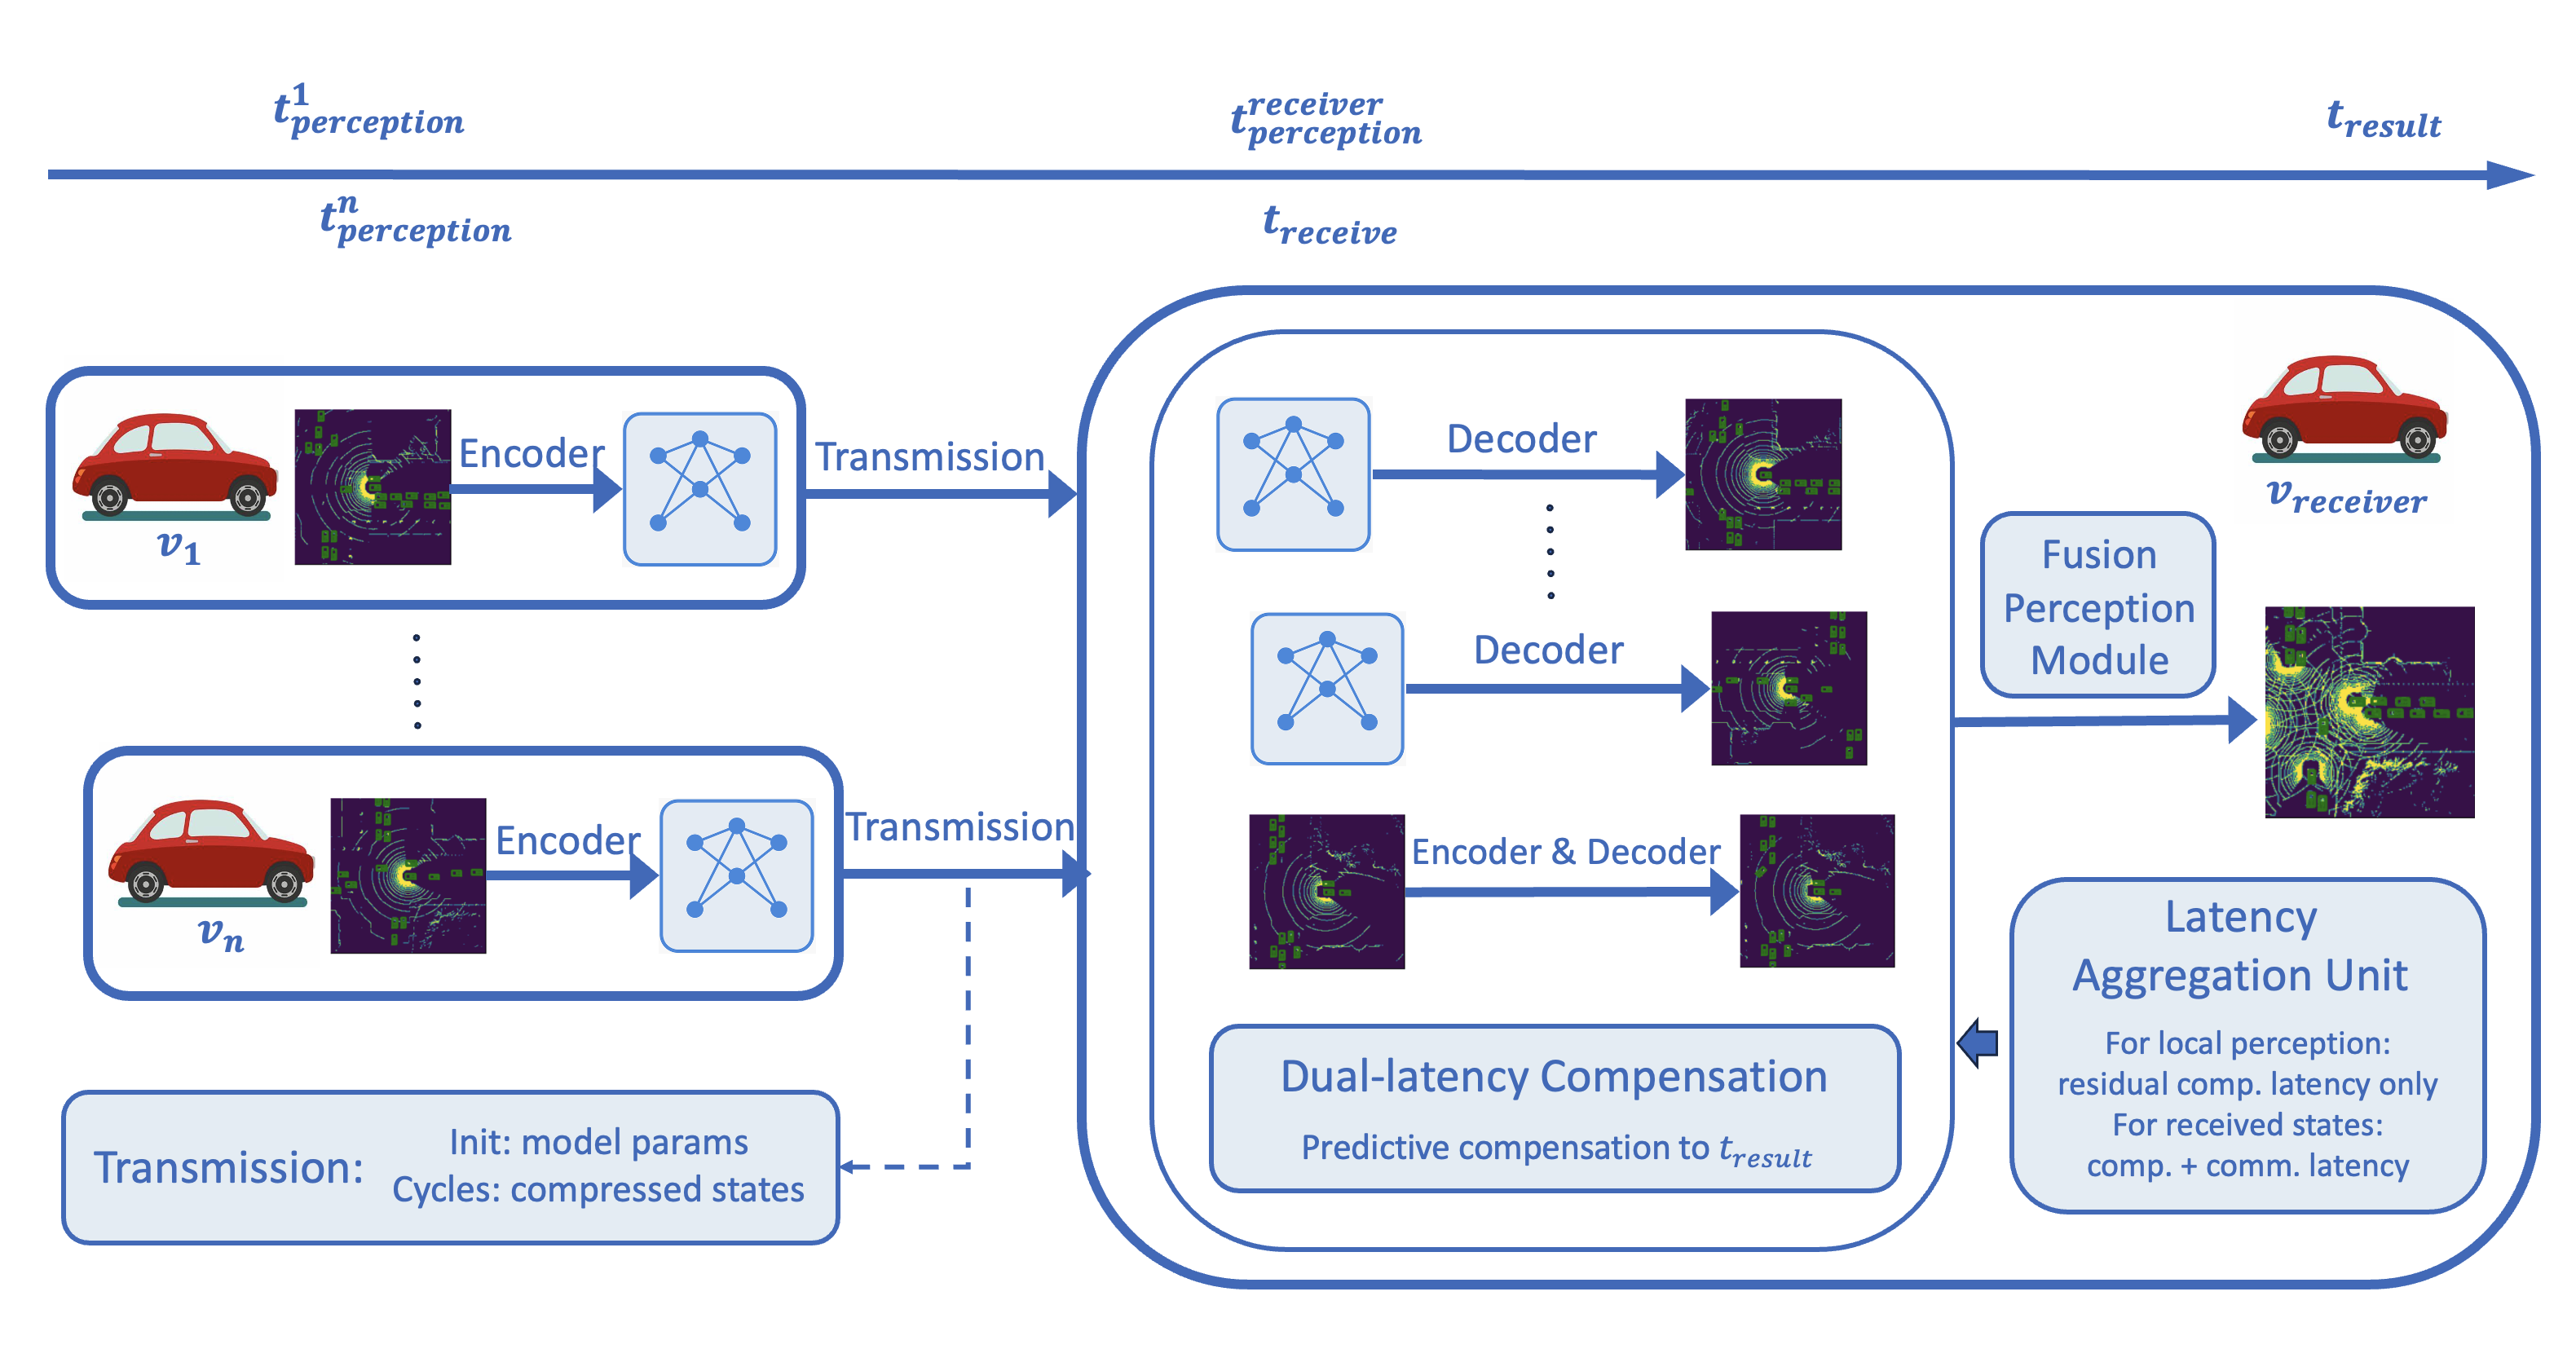
\includegraphics[width=7in]{figure2.png}
\caption{\textbf{Framework of dual-latency prediction compensation mechanism based on the
transmitter model.} 
$t^{n}_{perception}$ denotes the perception time of the $n$-th transmitting vehicle; 
    $t_{receive}$ is the time when the receiver obtains the last transmitted state; 
    $t^{receiver}_{perception}$ indicates the receiver’s latest local perception time, which coincides with $t_{receive}$; 
    and $t_{result}$ represents the expected time when computation is completed and the final perception result is obtained. 
\\Each transmitting vehicle encodes its local perception and \textbf{transmits either }\textbf{model parameters (initial exchange) or compressed intermediate states (subsequent cycles)}. Upon reception, each transmitted state is decoded using the corresponding vehicle’s prediction model, and then compensated to $t_{result}$ by accounting for \textbf{both communication and computation latencies}. Simultaneously, when the last state is received, the receiver obtains its latest local perception at $t^{receiver}_{perception} = t_{receive}$, which is further compensated for the residual computation latency to reach $t_{result}$. Finally, all latency-compensated data are synchronized at $t_{result}$ and fused within the fusion perception module, yielding timely environmental awareness.}
\label{fig_2}
\end{figure*}




In this section, we present a cooperative perception framework that addresses both \emph{communication latency} and \emph{computation latency} through a \emph{Dual-Latency Prediction Compensation Mechanism} as shown in Figure~\ref{fig_2}. The proposed approach is built upon a \emph{Vehicle-Specific Prediction Model} deployed at the transmitting vehicle and an efficient \emph{Model State Transmission} protocol, enabling the receiver to reconstruct the transmitter's future perception results and perform latency-compensated fusion. The proposed mechanism significantly enhances the real-time performance and robustness of cooperative perception. The overall procedure of the proposed mechanism is summarized in Algorithm~\ref{alg:dual_latency}.






\subsection{Vehicle-Specific Prediction Model}
\label{subsec:vspm}

To exploit the transmitter’s rich vehicle-specific history while minimizing communication cost and receiver-side latency, we instantiate $\mathcal{M}_{\theta_i}$ as a lightweight encoder--decoder ConvLSTM trained offline on vehicle $i$’s logs. The model learns idiosyncratic motion and sensing patterns from historical data and exposes compact decoder states $(\mathbf{h}^i_t,\mathbf{c}^i_t)$ that align with the state-transmission interface in \S\ref{subsec:state} and the dual-latency compensation in \S\ref{subsec:fusion}. The perception representation is a binary bird’s-eye-view (BEV) occupancy grid, denoted as $X^i_t \in \{0,1\}^{H\times W}$. Unless otherwise specified, $X^i_t$ also serves as the training supervision $Y^i_t$.

\subsubsection{Model architecture}
We realize the temporal transition $f_{\theta_i}$ (cf.\ Eq.~\ref{eq:lstm_update}) with a single-layer ConvLSTM using $3{\times}3$ convolutions (unit padding) and hidden width $32$. 
An \emph{encoder} ConvLSTM consumes the history $\mathcal{X}^i_{1:T}=\{X^i_1,\dots,X^i_T\}$ and summarizes it into $(\mathbf{h}^i_T,\mathbf{c}^i_T)$, 
where $\mathbf{h}^i_T$ denotes the final hidden state capturing spatial-temporal features, and $\mathbf{c}^i_T$ is the cell state that preserves long-term temporal memory.
A matched \emph{decoder} ConvLSTM, initialized with $(\mathbf{h}^i_T,\mathbf{c}^i_T)$, rolls the state forward for $S$ horizons. 
During \emph{training at the transmitter}, the first decoder input is the last observed frame and subsequent inputs follow the scheduled-sampling policy described below (see \S\ref{subsec:vspm} ``Autoregressive decoding''). 
Readout $g_{\theta_i}$ is implemented by a lightweight occupancy head,
\emph{Conv}$(32{\to}32,\,3{\times}3)$ + ReLU followed by \emph{Conv}$(32{\to}1,\,1{\times}1)$ and a sigmoid,
which maps decoder states to calibrated per-pixel probabilities $\widehat{Y}^i_k \in [0,1]^{H\times W}$.
We keep the decoder’s states compact so that the \emph{compressed intermediate model states} $(\mathbf{h}^i_t,\mathbf{c}^i_t)$ can serve as a transmissible state payload in $\mathcal{P}^{i\rightarrow j}$ with negligible bandwidth.

\subsubsection{Transmissible state and rollout interface}
The decoder’s \emph{compressed intermediate model states} $(\mathbf{h}^i_s,\mathbf{c}^i_s)$, 
representing the hidden and cell states of the ConvLSTM, 
serve as the compact predictive state. 
Given the transmitted states at sender time $s$, the receiver uses the cached $\theta_i$ and a rollout operator $\mathcal{R}(\cdot,\cdot,\widehat{\Delta})$ 
to advance the states and decode the transmitter’s occupancy prediction at the receiver’s current time:
\begin{equation}
\begin{aligned}
(\mathbf{h}',\mathbf{c}') \;=\; \mathcal{R}\!\big((\mathbf{h}^i_s,\mathbf{c}^i_s),\,\widehat{\Delta}\big), 
\qquad
\widehat{Y}^{i\rightarrow j}_{t} \;=\; g_{\theta_i}(\mathbf{h}').
\end{aligned}
\label{eq:state_update_and_prediction}
\end{equation}

Here, $\mathcal{R}$ corresponds to an \emph{autoregressive ConvLSTM transition}: at each rollout step,
\begin{equation}
(\mathbf{h}_{s+k},\mathbf{c}_{s+k}) = f_{\theta_i}\!\big(\mathbf{h}_{s+k-1},\mathbf{c}_{s+k-1}\big),
\label{eq:lstm_update}
\end{equation}

reusing the decoder’s own predicted occupancy from the previous step instead of any ground-truth inputs.
On the receiver, $\mathcal{R}$ runs in \emph{free mode without external inputs}, 
i.e., no raw frame $X^i_s$ is required in the packet.

$\widehat{\Delta}$ aggregates communication and computation latencies as defined in \S\ref{subsec:fusion}. 
For implementation convenience in our experiments, we quantize sequences with a temporal step $\Delta\tau=0.2\,$s and advance $\mathcal{R}$ by the corresponding number of discrete steps.

\subsubsection{Autoregressive decoding (training-time)}
Decoding is autoregressive. To mitigate exposure bias, we employ scheduled sampling: early epochs feed ground-truth previous frames to the decoder, and the policy smoothly transitions to self-feeding predictions as training progresses. Validation and test always run in free mode (self-feeding only) to reflect deployment behavior (which matches the receiver-side rollout described above).







\subsubsection{Training objectives}

\paragraph{Per-pixel dynamic weights}
For each pixel $(u,v)$, we define the dynamic mask and weights as:
\begin{align}
D^i_k(u,v) &= \mathbf{1}\!\left(X^{i,\mathrm{prev}}_k(u,v) \neq Y^i_k(u,v)\right), \\
w^i_k(u,v) &= 1 + \lambda_d\, D^i_k(u,v),
\label{eq:dynmask_weights_pixel}
\end{align}
where $X^{i,\mathrm{prev}}_k$ is the previous-frame input to the decoder at step $k$, and $\lambda_d \ge 0$ controls the emphasis on dynamic pixels. Setting $\lambda_d=0$ reduces to uniform weighting. During training with scheduled sampling,
$X^{i,\mathrm{prev}}_k \;=\; \alpha_k\,Y^i_{k-1} + (1-\alpha_k)\,\widehat{Y}^i_{k-1},$
where $\alpha_k\in\{0,1\}$ follows the schedule.
This weighting scheme highlights regions with motion changes, improving predictive performance on dynamic objects.

\paragraph{Dynamic binary cross-entropy (BCE)}
The BCE loss measures per-pixel occupancy prediction fidelity, enhanced with dynamic motion-aware weighting:
\begin{align}
&\mathrm{BCE}(\widehat{Y}^i_k, Y^i_k;\, w^i_k)
= - \frac{1}{HW} \sum_{u=1}^{H} \sum_{v=1}^{W} w^i_k(u,v) \notag \\
&\qquad \times \Bigl[
    Y^i_k(u,v) \cdot \log \widehat{Y}^i_k(u,v) \notag \\
&\quad + \big(1-Y^i_k(u,v)\big) \cdot \log \big(1-\widehat{Y}^i_k(u,v)\big)
\Bigr].
\label{eq:bce_loss}
\end{align}

\paragraph{Dice loss}
To address class imbalance in sparse occupancy grids, we employ the Dice coefficient loss:
\begin{align}
\mathrm{Dice}(\widehat{Y}^i_k, Y^i_k)
= 1 - \frac{2 \sum\limits_{u,v} \widehat{Y}^i_k(u,v) \, Y^i_k(u,v) + \epsilon}
              {\sum\limits_{u,v} \widehat{Y}^i_k(u,v) + \sum\limits_{u,v} Y^i_k(u,v) + \epsilon},
\label{eq:dice_loss}
\end{align}
where $\epsilon$ is a small constant ($10^{-6}$) for numerical stability. The Dice loss directly optimizes the overlap between predicted and true occupancy masks, especially benefiting underrepresented dynamic regions.

\paragraph{Curriculum warmup for auxiliary losses}  
To stabilize the early stage of training, we adopt a curriculum warmup strategy for the Dice loss only. Let $e$ denote the current training epoch (starting from $1$). During the initial $E_{\mathrm{warm}}$ epochs, we optimize only the dynamic-weighted BCE loss defined in Eq.~\eqref{eq:bce_loss}. After the warmup stage, the Dice loss term is gradually introduced over an additional $E_{\mathrm{ramp}}$ epochs by increasing its coefficient with a compact schedule:
\[
\lambda_{\mathrm{dice}}(e) \;=\; \lambda_{\mathrm{dice}}^\ast \cdot \min\!\Bigl\{1,\;\max\!\bigl\{0,\;\tfrac{e-E_{\mathrm{warm}}}{E_{\mathrm{ramp}}}\bigr\}\Bigr\}.
\]
Beyond $E_{\mathrm{warm}} + E_{\mathrm{ramp}}$ epochs, the Dice weight remains fixed at $\lambda_{\mathrm{dice}}^\ast$.

\paragraph{Training loss}
Our final per-step training loss is defined as:
\begin{align}
\mathcal{L}^i_k
&=\;
\underbrace{\mathrm{BCE}\!\left(\widehat{Y}^i_k, Y^i_k; w^i_k\right)}_{\text{occupancy prediction}}
\;+\;
\lambda_{\mathrm{dice}}(e)\,
\mathrm{Dice}\!\left(\widehat{Y}^i_k, Y^i_k\right).
\label{eq:final_loss}
\end{align}
The sequence-level objective averages the horizon-wise losses:
\[
\mathcal{L}^i = \frac{1}{S}\sum_{k=1}^{S}\mathcal{L}^i_k.
\]

\subsubsection{Training protocol}
We optimize with AdamW (learning rate $10^{-3}$), batch size $8$, for $30$ epochs. Data augmentation applies horizontal flips and $180^\circ$ rotations with probability $0.5$ to both history and targets. Inputs are rasterized from sparse $(y,x)$ indices into $H{\times}W$ binary grids (default $256{\times}256$). Encoder/decoder ConvLSTMs use hidden width $32$ and $3{\times}3$ kernels; validation is logged per horizon in free-running mode.
%In deployment, the transmitter runs the encoder/decoder online, transmits the \emph{compressed intermediate model states} $(\mathbf{h}^i_t,\mathbf{c}^i_t)$ (with timestamp and pose) as the compact state, and the receiver reconstructs $\widehat{Y}^i_{t}$ via Eq.~\eqref{eq:vspm_rollout_interface} using horizon $\widehat{\Delta}$, ensuring consistency with the dual-latency compensation pipeline in \S\ref{subsec:fusion}.






\subsection{Model State Transmission}
\label{subsec:state}

\subsubsection{One-Time Model Parameter Transmission}
During the initial vehicle-to-vehicle (V2V) communication, vehicle $i$ transmits its trained model parameters $\theta_i$ to the receiver. These parameters are sent only once and reused for all subsequent interactions, avoiding repeated transmission of large model parameters or feature tensors.

\subsubsection{Lightweight State Updates}
In subsequent communication cycles, the transmitting vehicle \(i\) no longer sends raw perception data or high-dimensional feature maps to the receiving vehicle \(j\). 
Instead, it transmits only the \emph{compressed intermediate model states}, defined as the decoder’s hidden and cell states \((\mathbf{h}^i_{t_{\text{per}}},\mathbf{c}^i_{t_{\text{per}}})\), along with the sender perception timestamp and pose:
\begin{equation}
    \mathcal{P}^{i \rightarrow j}(t_{\text{per}}\!\to\!t) 
    = \{\mathbf{h}^i_{t_{\text{per}}}, \mathbf{c}^i_{t_{\text{per}}}, t_{\text{per}}, \mathbf{T}^i_{t_{\text{per}}}\},
\end{equation}
where \(\mathbf{h}^i_{t_{\text{per}}}\) and \(\mathbf{c}^i_{t_{\text{per}}}\) are the decoder’s hidden and cell states at the sender's perception time \(t_{\text{per}}\), 
\(\mathbf{T}^i_{t_{\text{per}}}\) is the sender’s ego pose at the same moment, and \(t\) denotes the receiver time when the packet is received.
Here, \(t_{\text{per}}\) specifically indicates the timestamp when the transmitting vehicle \(i\) perceived the input data used to compute the transmitted states.
We refer to \((\mathbf{h}^i_{t_{\text{per}}},\mathbf{c}^i_{t_{\text{per}}})\) collectively as the \emph{compressed intermediate model states} since they provide a compact yet sufficient representation for prediction continuation. 
This design greatly reduces bandwidth usage while preserving the information necessary for accurate future prediction on the receiver side. 

% \paragraph{Advantages of Sending Compressed Intermediate States}
% Sending \emph{compressed intermediate model states} instead of raw perception data provides three main benefits:

% \begin{itemize}
%     \item \textbf{Efficient Computation:}  
%     If the sender transmits raw data, each receiver must independently complete the full prediction, causing redundant computation.  
%     By letting the sender perform most of the prediction process and sharing only intermediate states, receivers only compute the remaining latency-compensation steps, reducing overall computational load.

%     \item \textbf{Better Prediction with Less Data:}  
%     Intermediate states already encode sufficient historical context.  
%     This avoids the need to transmit large volumes of past sensor data while still enabling receivers to achieve accurate predictions, even during the first-time communication.

%     \item \textbf{Lower Communication Overhead:}  
%     Compared to raw frames or high-dimensional features, compressed states are much smaller, significantly reducing bandwidth usage while preserving essential temporal information.
% \end{itemize}






\begin{algorithm}[t]
\caption{Dual-latency Prediction Compensation with Vehicle-Specific Prediction Model (VSPM)}
\label{alg:dual_latency}
\begin{algorithmic}[1]

    \Require Transmitting vehicles \ensuremath{\mathcal{V}}, receiver \ensuremath{\mathrm{re}}
    \Require Cached parameters \ensuremath{\{\theta_i\}}, received packets \ensuremath{\{\mathcal{P}^{i\rightarrow\mathrm{re}}\}}
    \Require Local compressed states \ensuremath{(\mathbf{h}^{\mathrm{re}}_{t^{\mathrm{re}}_{\mathrm{per}}}, \mathbf{c}^{\mathrm{re}}_{t^{\mathrm{re}}_{\mathrm{per}}})}
    \Require Local model parameters \ensuremath{\theta_{\mathrm{re}}}, quantization step \ensuremath{\Delta\tau}

    \Ensure Latency-compensated fused occupancy prediction \ensuremath{\widehat{Y}^{\mathrm{re},\mathrm{fused}}_{t_{\mathrm{result}}}}

    \State \textbf{Initialization:} Each transmitting vehicle \ensuremath{i} sends \ensuremath{\theta_i} once; the receiver caches them.

    \State \textbf{Step 1: Packet Reception}
    \State Receive valid compressed packets at \ensuremath{t_{\mathrm{receive}}}:
    \Statex \hspace{\algorithmicindent}%
    \ensuremath{\mathcal{P}^{i\rightarrow\mathrm{re}}
      = \{\mathbf{h}^i_{t^i_{\mathrm{per}}},\; \mathbf{c}^i_{t^i_{\mathrm{per}}},\; t^i_{\mathrm{per}},\; \mathbf{T}^i_{t^i_{\mathrm{per}}}\}}
    \State Define $\mathcal{N}(\mathrm{re}) = \{\, i \in \mathcal{V} \mid \mathrm{re} \text{ receives a packet from } i \,\}$


    \State \textbf{Step 2: Unified Prediction Time}
    \State Compute \ensuremath{t_{\mathrm{result}} = t_{\mathrm{receive}} + \tau^{\mathrm{re}}_{t_{\mathrm{receive}}}}
    % \State Set waiting time \ensuremath{\delta^{\mathrm{wait}} = \max(0,\; t^{\mathrm{re}}_{\mathrm{start}} - t_{\mathrm{receive}})}

    \State \textbf{Step 3: Remote Branch Rollout}
    \ForAll{\ensuremath{i \in \mathcal{N}(\mathrm{re})}}
        \State \ensuremath{\widehat{\Delta}^{(i)} = t_{\mathrm{result}} - t^i_{\mathrm{per}}}
        %+ \delta^{\mathrm{wait}}}
        \State \ensuremath{K^{(i)} = \max\{0,\; \mathrm{round}(\widehat{\Delta}^{(i)}/\Delta\tau)\}}
        \State \ensuremath{(\mathbf{h}',\mathbf{c}') \gets \mathcal{R}\bigl((\mathbf{h}^i_{t^i_{\mathrm{per}}}, \mathbf{c}^i_{t^i_{\mathrm{per}}}),\; K^{(i)}\bigr)}
        \State \ensuremath{\widehat{Y}^{i\rightarrow\mathrm{re}}_{t_{\mathrm{result}}} = g_{\theta_i}(\mathbf{h}')}
    \EndFor

    \State \textbf{Step 4: Local Branch Rollout}
    \State \ensuremath{\widehat{\Delta}_{\mathrm{re}} = t_{\mathrm{result}} - t^{\mathrm{re}}_{\mathrm{per}}}
    \State \ensuremath{K_{\mathrm{re}} = \max\{0,\; \mathrm{round}(\widehat{\Delta}_{\mathrm{re}}/\Delta\tau)\}}
    \State \ensuremath{(\mathbf{h}',\mathbf{c}') \gets \mathcal{R}\bigl((\mathbf{h}^{\mathrm{re}}_{t^{\mathrm{re}}_{\mathrm{per}}}, \mathbf{c}^{\mathrm{re}}_{t^{\mathrm{re}}_{\mathrm{per}}}),\; K_{\mathrm{re}}\bigr)}
    \State \ensuremath{\widehat{Y}^{\mathrm{re}}_{t_{\mathrm{result}}} = g_{\theta_{\mathrm{re}}}(\mathbf{h}')}

    \State \textbf{Step 5: Spatio-Temporal Alignment}
    \ForAll{\ensuremath{i \in \mathcal{N}(\mathrm{re})}}
        \State Transform \ensuremath{\widehat{Y}^{i\rightarrow\mathrm{re}}_{t_{\mathrm{result}}}} into the receiver frame
        \Statex \hspace{\algorithmicindent}using \ensuremath{\mathbf{T}^i_{t^i_{\mathrm{per}}}} and \ensuremath{\mathbf{T}^{\mathrm{re}}_{t_{\mathrm{result}}}}
    \EndFor

    \State \textbf{Step 6: Confidence-Aware Fusion}
    \State $\displaystyle
        \widehat{Y}^{\mathrm{re},\mathrm{fused}}_{t_{\mathrm{result}}}
        = \mathcal{F}\!\Bigl(
            \widehat{Y}^{\mathrm{re}}_{t_{\mathrm{result}}},
            \{\widehat{Y}^{i\rightarrow\mathrm{re}}_{t_{\mathrm{result}}}\}_{i\in\mathcal{N}(\mathrm{re})}
        \Bigr)
    $

    \State \textbf{Step 7: Output and Buffer Update}
    \State Publish \ensuremath{\widehat{Y}^{\mathrm{re},\mathrm{fused}}_{t_{\mathrm{result}}}} and discard outdated packets

\end{algorithmic}
\end{algorithm}











\subsection{Dual-Latency Predictive Compensation Fusion}
\label{subsec:fusion}
\subsubsection{Computation-latency Estimation}
We define, for vehicle $i$ at time $t$, the elapsed runtime required to (i) process all \emph{compressed state packets} currently stored in its receive buffer together with its own local state, and (ii) compute the final \emph{fused} perception result as $\tau^i_t$. This computation time can be estimated from the vehicle's current computing-unit status and the volume of pending tasks; thus, $\tau^i_t$ can be approximated using an empirical formula. 

\subsubsection{Latency-Aware Prediction}
We describe the procedure from the receiver's perspective. Consider a sender $i$ and a receiver vehicle \emph{receiver}. Let $\mathcal{P}^{i \rightarrow \text{re}}(t^{i}_{\text{per}}\!\to\!t_{\text{receive}})$ represent a compressed state packet generated by sender $i$ at perception time $t^{i}_{\text{per}}$ and received by the \emph{receiver} vehicle at time $t_{\text{receive}}$. The receiver aims to produce a prediction aligned with:
\[
t_{\text{result}} \;=\; t_{\text{receive}} \,+\, \tau^{\text{re}}_{t_{\text{receive}}}.
\]
The corresponding total latency-compensation horizon is given by:
\[
\widehat{\Delta} \;=\; t_{\text{result}} \,-\, t^{i}_{\text{per}}.
\]
%If multiple sender vehicles are present or if packets experience additional waiting time in the receiver buffer before being processed, we add this waiting time to the effective horizon. Specifically, if fusion starts at $t^{\text{re}}_{\text{start}} \ge t_{\text{receive}}$, we define $\delta^{\text{wait}} = t^{\text{re}}_{\text{start}} - t_{\text{receive}}$ and update $\widehat{\Delta} \leftarrow \widehat{\Delta} + \delta^{\text{wait}}$ accordingly.

Using the cached model parameters $\theta_i$ and the \emph{compressed intermediate model states} $(\mathbf{h}^i_{t^{i}_{\text{per}}}, \mathbf{c}^i_{t^{i}_{\text{per}}})$ contained in the packet, the receiver rolls the model forward in free mode by $\widehat{\Delta}$ with the rollout operator $\mathcal{R}(\cdot)$ introduced in \S\ref{subsec:vspm}, and decodes the occupancy prediction aligned to $t_{\text{result}}$:
\[
(\mathbf{h}',\mathbf{c}') \;=\; \mathcal{R}\!\Big((\mathbf{h}^i_{t^{i}_{\text{per}}}, \mathbf{c}^i_{t^{i}_{\text{per}}}),\,\widehat{\Delta}\Big), 
\qquad
\widehat{Y}^{i\rightarrow \text{re}}_{t_{\text{result}}} \;=\; g_{\theta_i}(\mathbf{h}').
\]


\subsubsection{Local Latency Compensation}
In parallel, the receiver compensates for its own computation latency by propagating its most recent local perception at time $t^{\text{re}}_{\text{per}}$ forward to the unified prediction time $t_{\text{result}}$. We define the local latency-compensation horizon as:
\[
\widehat{\Delta}_{\text{re}} \;=\; t_{\text{result}} - t^{\text{re}}_{\text{per}}.
\]
Using the cached local model parameters $\theta_{\text{re}}$ and the \emph{compressed intermediate model states} $(\mathbf{h}^{\text{re}}_{t^{\text{re}}_{\text{per}}}, \mathbf{c}^{\text{re}}_{t^{\text{re}}_{\text{per}}})$, the receiver similarly performs free-mode rollout:
\[
(\mathbf{h}',\mathbf{c}') \;=\; \mathcal{R}\!\Big((\mathbf{h}^{\text{re}}_{t^{\text{re}}_{\text{per}}}, \mathbf{c}^{\text{re}}_{t^{\text{re}}_{\text{per}}}),\,\widehat{\Delta}_{\text{re}}\Big), 
\qquad
\widehat{Y}^{\text{re}}_{t_{\text{result}}} \;=\; g_{\theta_{\text{re}}}(\mathbf{h}').
\]
Thus, both the local and remote predictions are aligned to the same global time $t_{\text{result}}$, enabling subsequent spatio-temporal alignment and multi-vehicle fusion.


\subsubsection{Spatio-Temporal Alignment and Fusion}
To integrate multi-vehicle perception, each reconstructed remote prediction $\widehat{Y}^{i \rightarrow \text{re}}_{t_{\text{result}}}$ is transformed into the receiver’s coordinate frame using the sender’s ego pose $\mathbf{T}^i_{t^{i}_{\text{per}}}$ and the receiver’s ego pose $\mathbf{T}^{\text{re}}_{t_{\text{result}}}$.  
Before fusion, both local and remote predictions are temporally aligned at the unified prediction time $t_{\text{result}}$.  
We then apply a confidence-aware spatio-temporal fusion strategy that combines the compensated local prediction $\widehat{Y}^{\text{re}}_{t_{\text{result}}}$ with all latency-compensated remote predictions:
\begin{equation}
    \widehat{Y}^{\text{re},\mathrm{fused}}_{t_{\text{result}}}
    = \mathcal{F}\!\Big(
        \widehat{Y}^{\text{re}}_{t_{\text{result}}},\,
        \{\widehat{Y}^{i \rightarrow \text{re}}_{t_{\text{result}}}\}_{i \in \mathcal{N}(\text{re})}
    \Big),
\end{equation}
where $\mathcal{F}(\cdot)$ denotes a generic perception fusion operator, providing flexibility to integrate any fusion model.  
Here, $\mathcal{N}(\text{re})$ represents the set of all transmitting vehicles from which the receiver \text{re} has successfully received valid compressed state packets during the current fusion cycle.  
In our experiments, we instantiate $\mathcal{F}$ with V2VNet\cite{wang2020v2vnet} and DiscoNet\cite{li2021learning} fusion head adapted to operate on occupancy probabilities; other strategies can also be seamlessly integrated.


% \subsection{Dual-Latency Compensation and Confidence-Aware Fusion}

% The overall procedure of the proposed Dual-latency Prediction Compensation with Vehicle-Specific Prediction Model (VSPM) is summarized in Algorithm~\ref{alg:dual_latency}. The algorithm first initializes cached vehicle-specific parameters and receives compressed packets from neighboring vehicles. Then, a unified prediction time is determined to synchronize local and remote predictions. For each received packet, the remote branch performs latent state rollout to compensate for communication and processing latencies, while the local branch predicts its own occupancy at the same unified time. Afterward, all remote predictions are transformed into the receiver’s coordinate frame, and a confidence-aware spatio-temporal fusion strategy integrates both local and remote results to produce the final latency-compensated fused occupancy prediction.
